\section{Evaluation}
\label{sec:evaluation}

The evaluation answers four questions.
\textbf{Q1}: Do agent metadata keys predict routed expert working sets?
\textbf{Q2}: How much do \RouteSig predictions improve prefetch, scheduling, and placement replay?
\textbf{Q3}: Can the requested \Qwen model run through real vLLM with the \project sidecar?
\textbf{Q4}: Does the dense-model fallback remain explicit, measured, and reproducible?

\subsection{Setup}
\label{sec:eval-setup}

The workload contains 216 normalized agent subrequests from five workflow families: planner-coder-tester, search-summarize, tool-use, multi-agent discussion, and SWE-agent code repair.
For routed MoE evidence, we use \TinyMixtral through real Transformers router logits and collect 80 routed traces.
For the requested end-to-end serving experiment, we use \Qwen at the local path \texttt{/home/youwei/bzh/model/Qwen/Qwen2.5-7B-Instruct} with real vLLM.

The \Qwen experiment runs baseline and \texttt{tokenmoe\_sidecar} modes over batch sizes 1, 2, 4, and 8.
Each mode records raw generations, request metadata, per-request latency, output token count, sidecar decision time, model capability, vLLM version, CUDA device selection, and shard logs.
The experiment is resumable because a long vLLM process can be interrupted by shared GPU contention.

\subsection{Agent-Conditioned MoE Locality (Q1)}
\label{sec:eval-locality}

\begin{figure*}[t]
\centering
\begin{subfigure}{0.32\linewidth}
\centering
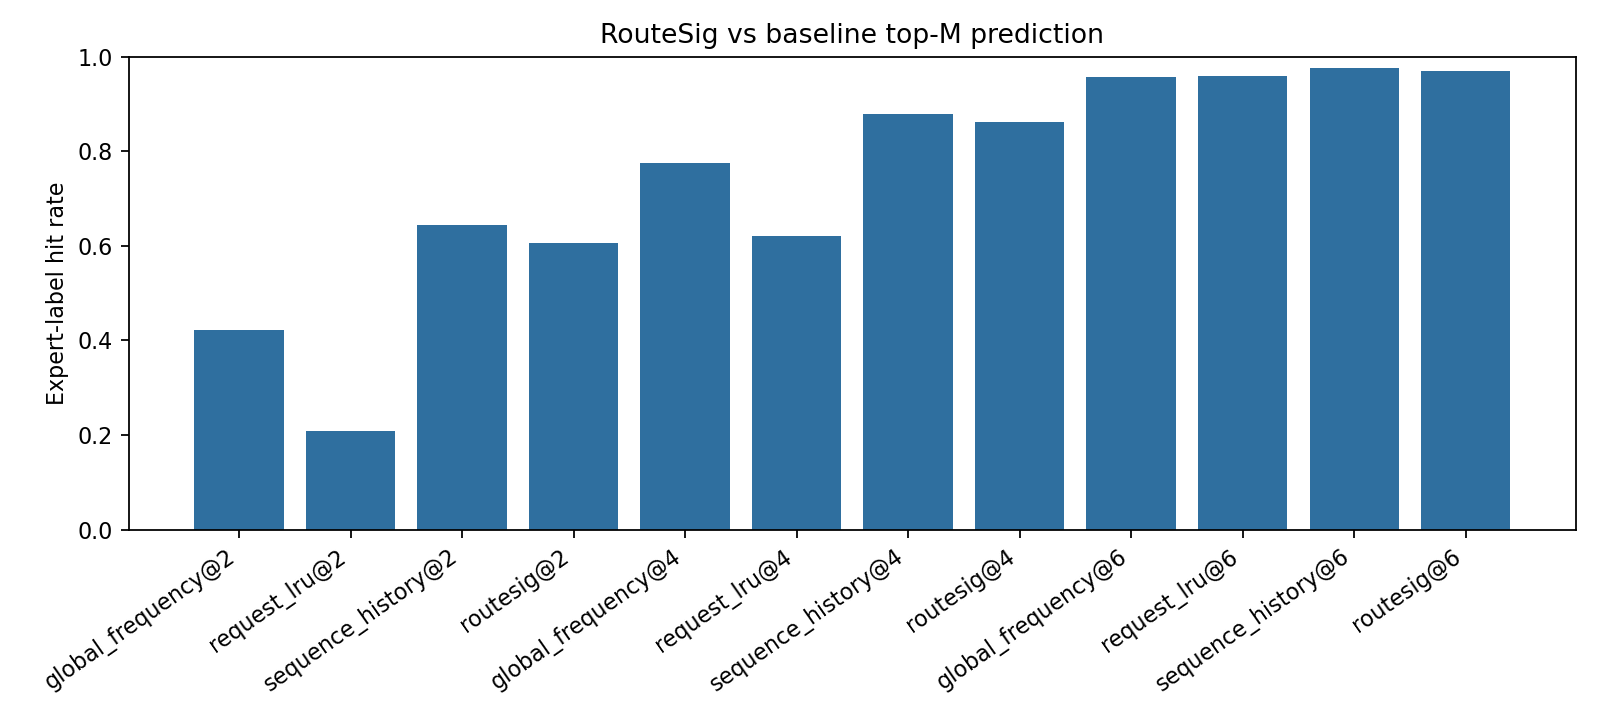
\includegraphics[width=\linewidth]{img/exp/topm_hit_rate.png}
\caption{Top-$M$ hit rate}
\end{subfigure}
\hfill
\begin{subfigure}{0.32\linewidth}
\centering
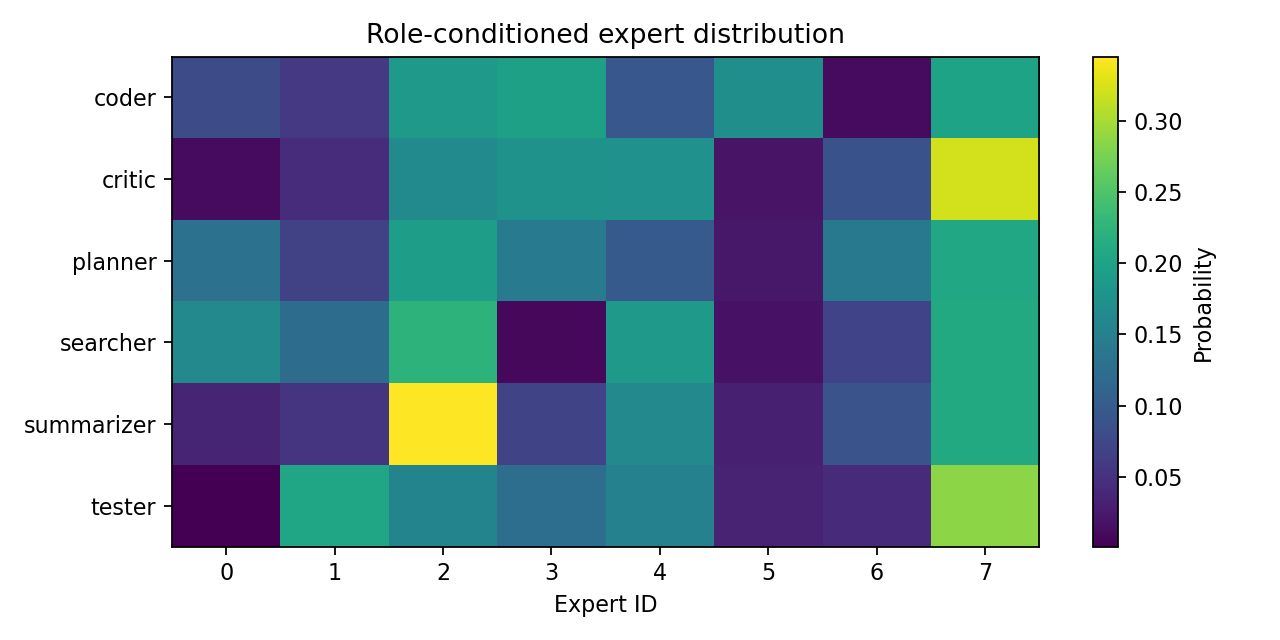
\includegraphics[width=\linewidth]{img/exp/role_expert_heatmap.png}
\caption{Role/expert heatmap}
\end{subfigure}
\hfill
\begin{subfigure}{0.32\linewidth}
\centering
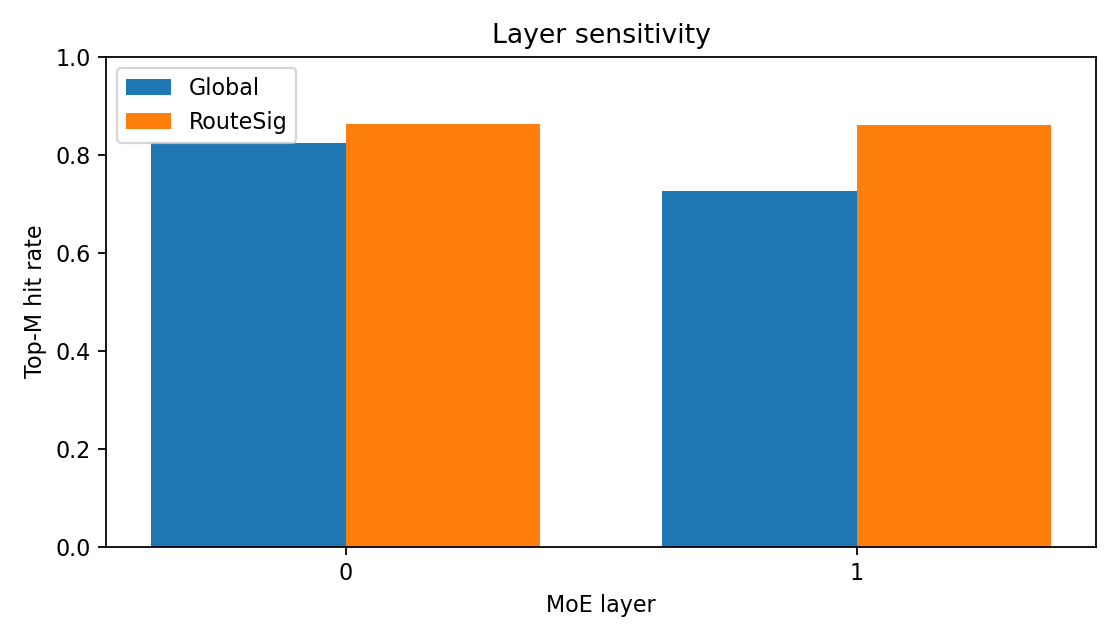
\includegraphics[width=\linewidth]{img/exp/layer_sensitivity.png}
\caption{Layer sensitivity}
\end{subfigure}
\caption{
Real routed traces from \TinyMixtral show that agent metadata predicts expert working sets.
\RouteSig improves top-4 hit rate over global frequency and especially helps the second routed layer.
}
\label{fig:locality}
\end{figure*}

Table~\ref{tab:routesig} summarizes the routed-trace result.
At top-4, \RouteSig reaches 86.1\% expert-label hit rate, compared with 77.4\% for global frequency.
The gain is not uniform across layers: layer 0 improves from 82.3\% to 86.3\%, while layer 1 improves from 72.5\% to 86.0\%.
This supports the core hypothesis that request metadata adds information beyond a global expert popularity prior.

\begin{table}[t]
\centering
\caption{Top-$M$ routed expert hit rates on 80 real \TinyMixtral traces.}
\label{tab:routesig}
\begin{tabular}{lccc}
\toprule
Predictor & Top-2 & Top-4 & Top-6 \\
\midrule
Global frequency & 42.1\% & 77.4\% & 95.7\% \\
Request LRU & 20.9\% & 62.2\% & 95.8\% \\
Sequence history & 64.3\% & 87.9\% & 97.6\% \\
\RouteSig & 60.6\% & 86.1\% & 96.9\% \\
\bottomrule
\end{tabular}
\end{table}

\subsection{Replay Impact (Q2)}
\label{sec:eval-replay}

\begin{figure}[t]
\centering
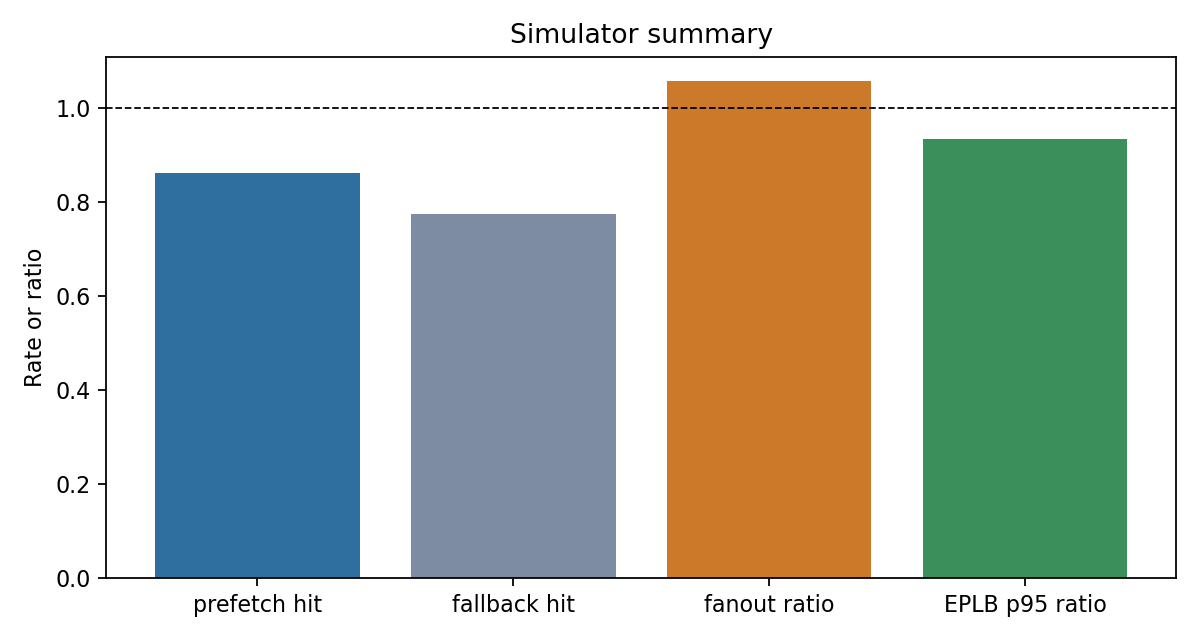
\includegraphics[width=\columnwidth]{img/exp/simulator_summary.png}
\Description{A bar chart summarizes prefetch, scheduler, and EPLB replay metrics.}
\caption{
Replay simulators translate \RouteSig predictions into serving-policy proxies.
They estimate prefetch opportunity, dependency-safe scheduling behavior, and EPLB-style placement improvement.
}
\label{fig:simulator}
\end{figure}

The prefetch replay estimates an 86.1\% hit rate, a 2.1\% wasted-prefetch rate, and 160.4 ms of stall-reduction proxy.
The scheduling replay forms dependency-safe batches with zero dependency violations.
The EPLB replay reduces p95 tail load from 585.0 to 546.4 tokens and p99 tail load from 611.4 to 563.6 tokens.
These are not end-to-end speedups; they are policy-level estimates derived from exact routed traces.
They show where a production MoE runtime could use the same signal without changing router semantics.

\subsection{Real vLLM Qwen Run (Q3)}
\label{sec:eval-vllm}

\begin{table*}[t]
\centering
\caption{Real vLLM/\Qwen end-to-end run over 216 agent requests per mode and batch size. The model is dense, so routed-expert capture is disabled and the sidecar records explicit fallback decisions.}
\label{tab:vllm-summary}
\begin{tabular}{llrrrrr}
\toprule
Mode & Batch & Requests & Mean ms & P95 ms & Req/s & Sidecar us \\
\midrule
Baseline & 1 & 216 & 364.5 & 373.1 & 2.74 & 0.0 \\
Baseline & 2 & 216 & 181.4 & 186.8 & 5.51 & 0.0 \\
Baseline & 4 & 216 & 93.0 & 97.1 & 10.76 & 0.0 \\
Baseline & 8 & 216 & 48.9 & 49.8 & 20.45 & 0.0 \\
TokenMoE sidecar & 1 & 216 & 351.7 & 359.2 & 2.84 & 41.6 \\
TokenMoE sidecar & 2 & 216 & 181.5 & 187.3 & 5.51 & 42.7 \\
TokenMoE sidecar & 4 & 216 & 93.3 & 94.8 & 10.71 & 14.9 \\
TokenMoE sidecar & 8 & 216 & 48.9 & 49.8 & 20.44 & 10.0 \\
\bottomrule
\end{tabular}
\end{table*}


\begin{figure*}[t]
\centering
\begin{subfigure}{0.49\linewidth}
\centering
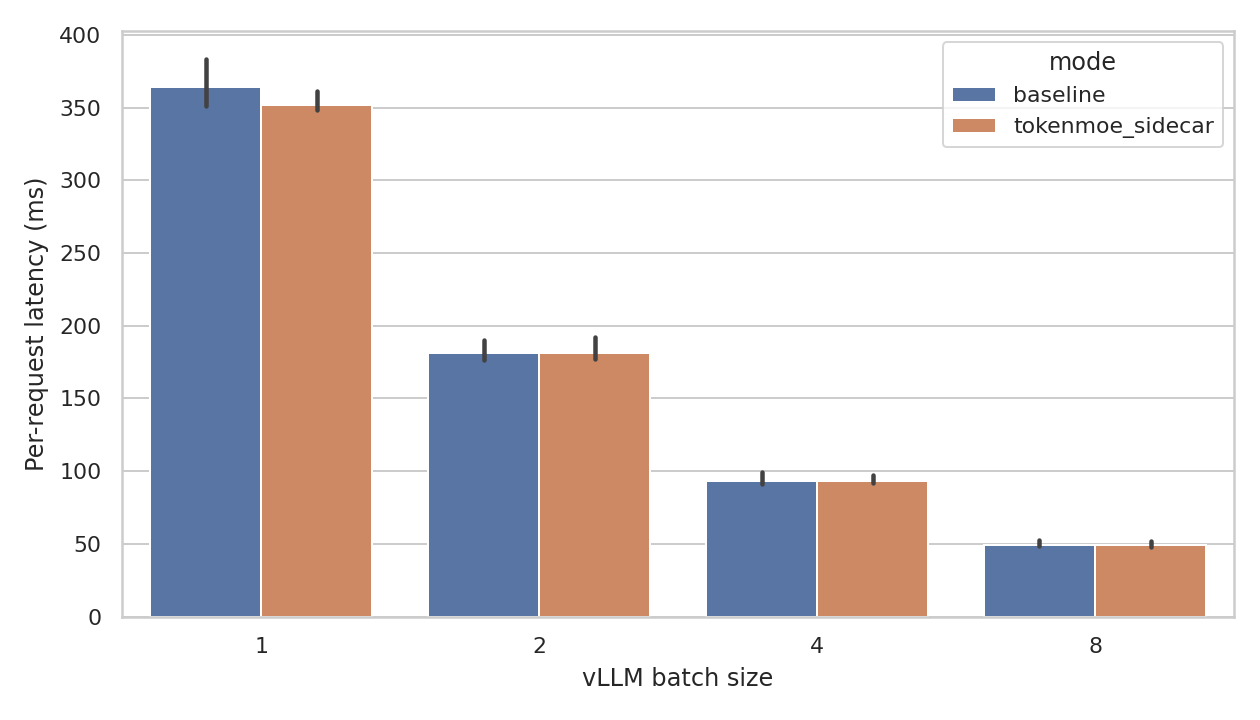
\includegraphics[width=\linewidth]{img/exp/latency_by_batch.png}
\caption{Latency by batch size}
\end{subfigure}
\hfill
\begin{subfigure}{0.49\linewidth}
\centering
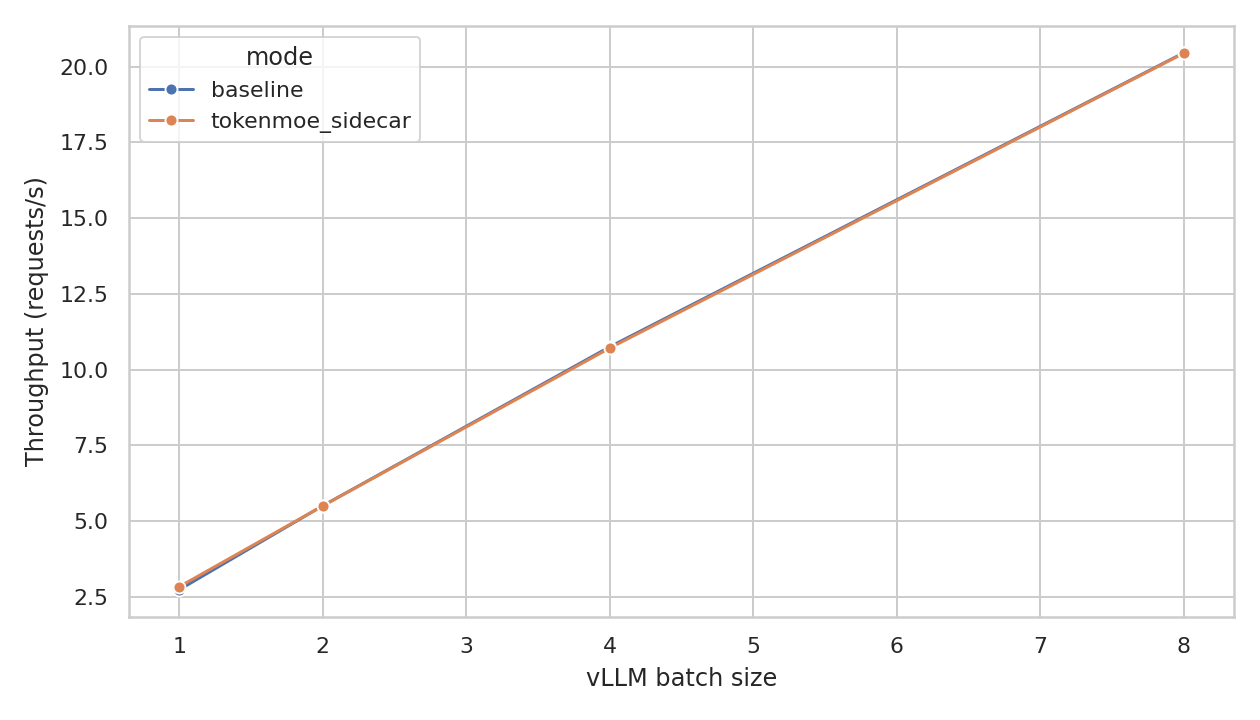
\includegraphics[width=\linewidth]{img/exp/throughput_by_batch.png}
\caption{Throughput by batch size}
\end{subfigure}
\caption{
Real vLLM run on the requested \Qwen model.
The target is dense, so the experiment measures serving integration and sidecar overhead rather than routed-expert speedup.
}
\label{fig:vllm-qwen-main}
\end{figure*}

\begin{figure}[t]
\centering
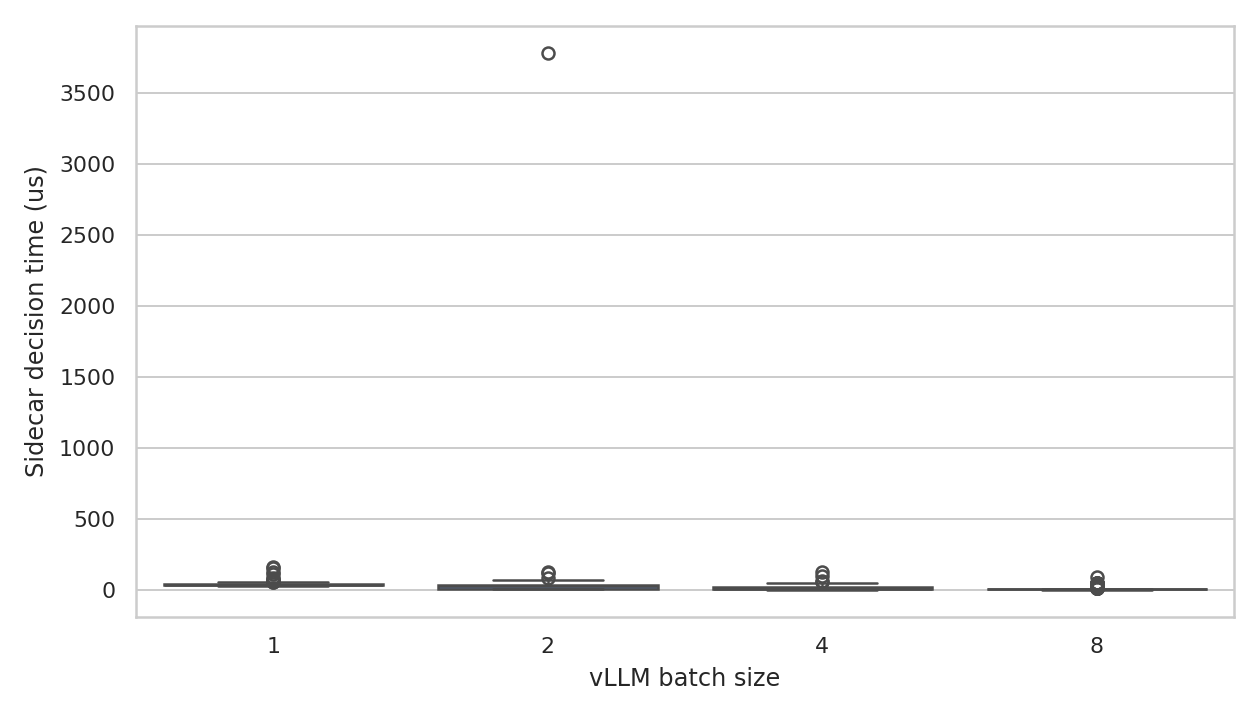
\includegraphics[width=\columnwidth]{img/exp/sidecar_overhead.png}
\Description{A box plot shows microsecond-scale sidecar decision overhead across batch sizes.}
\caption{
\project sidecar decision time in the dense \Qwen fallback path.
The sidecar records metadata hashes, fallback keys, and explicit fallback reason for every request.
}
\label{fig:sidecar-overhead}
\end{figure}

The \Qwen run validates the deployed path.
vLLM loads the local model, generates outputs for the full agent workload, and records every prompt and response.
The capability detector identifies the model as dense Qwen2 and sets \texttt{supports\_routed\_expert\_capture=false}.
Therefore all \texttt{tokenmoe\_sidecar} requests take the explicit \texttt{dense\_model\_no\_moe\_router} fallback.
This result is a negative MoE result but a positive systems result: the same serving sidecar runs end-to-end and refuses to claim unavailable routed traces.
The sidecar does not alter prompts, sampling parameters, or model weights.
We nevertheless report exact-output match as a measurement rather than a proof obligation because the full run uses independently restarted vLLM shards; batch execution is not bitwise stable across all shard and batch-size configurations.
Exact output match is 100\% for batch size 1 and 85.2--87.0\% for batch sizes 2--8.

\subsection{Reproducibility and Failures (Q4)}
\label{sec:eval-repro}

All experiment attempts are preserved.
The environment logs include the initial unresolved vLLM install, the corrected PyTorch/vLLM installation, the Transformers compatibility failure, and the final verified stack.
The vLLM logs include successful probe runs, a long-process cleanup hang after 60 baseline requests, two OOM failures caused by external GPU occupation, and the final resumable sharded run.
These failures are not hidden because they affect how the final experiment should be interpreted: the reported vLLM latency is a real shared-machine measurement with explicit resource provenance, not an isolated benchmark.
